\section{实验与结果分析}
\setchapternum{5}

\subsection{实验环境与设置}

实验基于 Python 与 PyTorch 框架，在单张 NVIDIA RTX 3060 GPU 上完成。严格遵循 MNIST 标准划分，在 $60{,}000$ 张训练样本上训练、在独立的 $10{,}000$ 张测试样本上评估，训练配置与第四章一致。

\subsection{评价指标}

本文采用准确率（式(\ref{eq:acc})）作为主要指标，并辅以精确率、召回率及其调和平均 F1 分数（式(\ref{eq:f1})）。对十个类别取宏平均以反映整体性能。

\begin{equation}
\mathrm{Accuracy} = \frac{TP + TN}{TP + TN + FP + FN}
\label{eq:acc}
\end{equation}

\begin{equation}
\mathrm{F1} = \frac{2 \times \mathrm{Precision} \times \mathrm{Recall}}{\mathrm{Precision} + \mathrm{Recall}}
\label{eq:f1}
\end{equation}

\subsection{结果与对比分析}

各方法在 MNIST 测试集上的准确率如表\ref{tab:comparison}所示。本文方法达到 $99.32\%$，显著优于线性的 Softmax 回归与全连接的多层感知机，并较经典的 LeNet-5\cite{lecun1998gradient}进一步提升，体现了卷积结构与训练优化策略的有效性\cite{goodfellow2016deep}。

\begin{table}[htbp]
\centering
\caption{不同方法在 MNIST 测试集上的准确率对比\\Table~\thetable\ Accuracy comparison of different methods on MNIST}
\label{tab:comparison}
\begin{tabular*}{\linewidth}{@{\extracolsep{\fill}}c c c}
\toprule
方法 & 测试准确率 (\%) & 备注 \\
\midrule
Softmax 回归 & 92.0 & 线性分类器 \\
多层感知机（MLP） & 98.1 & 全连接网络 \\
LeNet-5 & 98.9 & 经典卷积网络 \\
\textbf{本文方法} & \textbf{99.32} & 本文 CNN \\
\bottomrule
\end{tabular*}
\end{table}

\subsection{训练过程与错误分析}

训练损失与测试准确率随轮次的变化如图\ref{fig:curve}所示，模型在约第 $10\sim15$ 轮趋于收敛，训练与测试表现差距较小，无明显过拟合。测试集混淆矩阵如图\ref{fig:confusion}所示，绝大多数样本集中于对角线，错误主要发生在书写形近的数字对（如 $4$ 与 $9$、$3$ 与 $5$）之间。

\begin{figure}[htb]
\centering
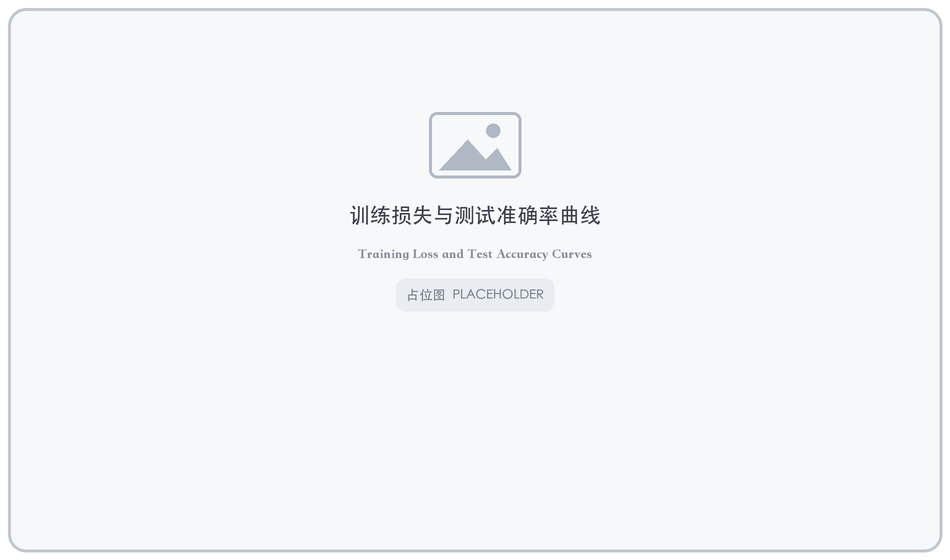
\includegraphics[width=0.85\linewidth]{figures/fig-training-curve.png}
\caption{训练损失与测试准确率曲线\\Fig.~\thefigure\ Training loss and test accuracy curves}
\label{fig:curve}
\end{figure}

\begin{figure}[htb]
\centering
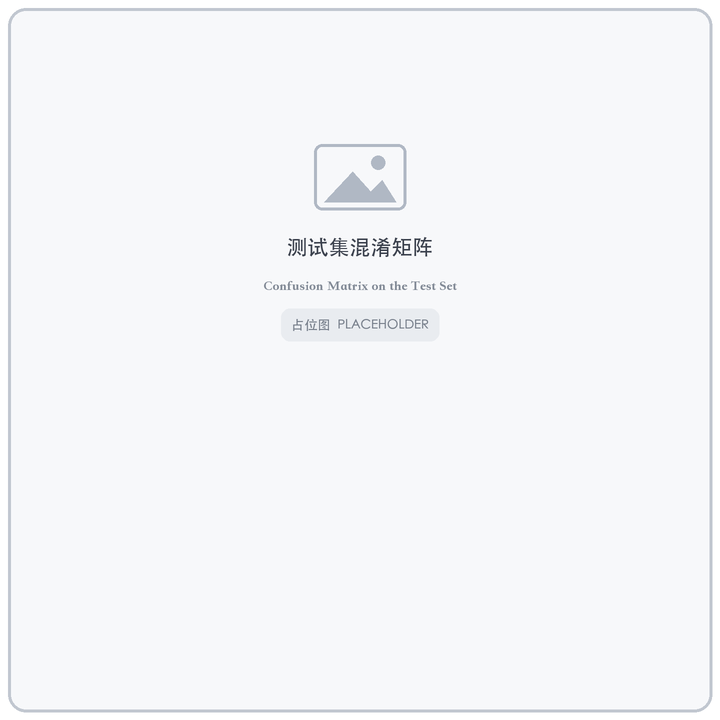
\includegraphics[width=0.7\linewidth]{figures/fig-confusion-matrix.png}
\caption{测试集混淆矩阵\\Fig.~\thefigure\ Confusion matrix on the test set}
\label{fig:confusion}
\end{figure}

\subsection{本章小结}

本章在 MNIST 数据集上验证了本文方法，测试准确率达 $99.32\%$，优于各对比方法，且收敛稳定、泛化良好。
